\documentclass{bksec}


\usetheme{bksec}


% The upstream template's \displayauthors (beamerinnerthemebksec.sty) drives
% its even-author loop with \foreach \i in {1, ..., \authornumeven}. When
% there's a single author, \authornumeven evaluates to 0 and pgffor's
% single-bound "1, ..., 0" range still fires one spurious iteration with an
% undefined image, aborting the build. Guarding that loop behind
% \ifnum\authornum>1 fixes the solo-author case without touching the shipped
% template files. Even/multi-author decks are unaffected.
\makeatletter
\renewcommand{\displayauthors}[1]{
    \def\authorinfopanewidth{.2\textwidth}
    \pgfmathsetmacro{\authornumeven}{2 * floor(\authornum / 2)}
    \def\logooffsetx{\logowidthhalf}

    \ifnum\authornum>1
        \foreach \i in {1, ..., \authornumeven} {
            \getauthorinfo{\i}

            \authorinfopaney{#1}{\i}

            \pgfmathsetmacro{\authorinfopanecolumn}{int(mod(\i, 2))}
            \ifnum\authorinfopanecolumn=1
                \node[
                    anchor=west,
                    minimum width=.25\paperwidth, minimum height=\logowidth
                ] (authorinfopane) at (#1.west |- authorinfopaney) {};
            \else
                \node[
                    anchor=east,
                    minimum width=.25\paperwidth, minimum height=\logowidth
                ] (authorinfopane) at (#1.east |- authorinfopaney) {};
            \fi

            \displaylogowithtext
                {authorinfopane.west}
                {\logooffsetx}{0}
                {authorpfp}
                {\authorpfp}
                {\tiny\bfseries}
                {Presenter \i: \authorrealname \\
                \textcolor{themecolor}{@\authornickname}}
        }
    \fi

    \pgfmathsetmacro\authornumisodd{int(mod(\authornum, 2))}
    \ifnum\authornumisodd=1
        \getauthorinfo{\authornum}

        \authorinfopaney{#1}{\authornum}
        \node[minimum width=.25\paperwidth, minimum height=\logowidth]
            (authorinfopane) at (#1.center |- authorinfopaney) {};

        \displaylogowithtext
            {authorinfopane.west}
            {\logooffsetx}{0}
            {authorpfp}
            {\authorpfp}
            {\tiny\bfseries}
            {Presenter \authornum: \authorrealname \\
            \textcolor{themecolor}{@\authornickname}}
    \fi
}
\makeatother


\begin{document}


\graphicspath{{./assets/presentation/}}


\title{Return by Death}
\subtitle{A Re:Zero-Themed CTF Challenge}
\thumbnail{rbd-thumbnail}
\author{haiyahhh-pfp}{Haiyahhh}{Haiyahhh}


\begin{frame}
    \titlepage
\end{frame}


\begin{frame}{Agenda}
    \tableofcontents
\end{frame}

\section{Concept}
    \begin{frame}{Theme \& Core Lesson}
        \begin{itemize}
            \item Re:Zero: die, reset, try again
            \item Four vulnerabilities, one chain
            \begin{itemize}
                \item DOM Clobbering
                \item TOCTOU race condition
                \item Kubernetes Pod lifecycle
                \item Insecure deserialization (PyYAML)
            \end{itemize}
            \item White/Gray-box: source \& manifests provided
        \end{itemize}
    \end{frame}

\section{Background You Need}
    \begin{frame}{Kubernetes 101}{Pods, volumes, policies}
        \begin{columns}[T]
            \begin{column}{.55\textwidth}
                \begin{itemize}
                    \item Container crash $\neq$ Pod deletion
                    \item \texttt{emptyDir} volume survives a container restart
                    \item \texttt{readOnlyRootFilesystem}: blocks webshells
                    \item \texttt{NetworkPolicy}: pod-level firewall
                \end{itemize}
            \end{column}
            \begin{column}{.4\textwidth}
                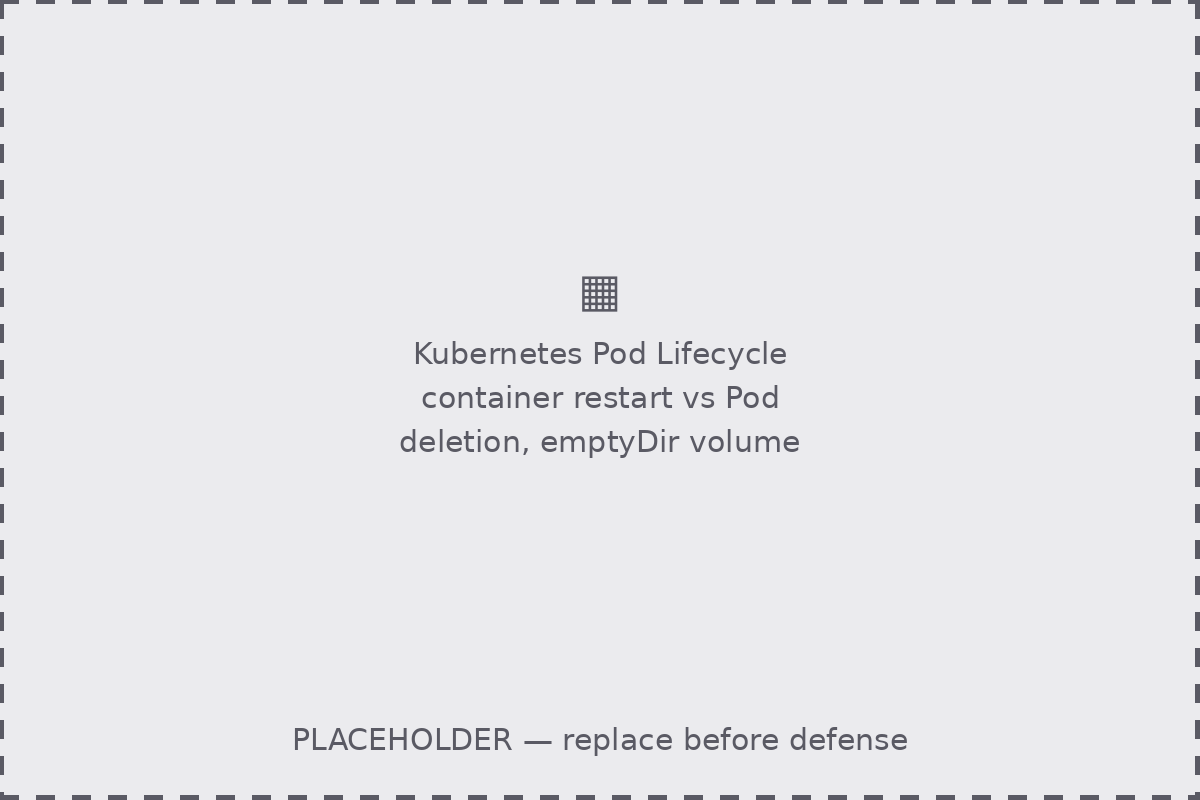
\includegraphics[width=\textwidth]{k8s-lifecycle-diagram.png}
            \end{column}
        \end{columns}
    \end{frame}

    \begin{frame}{TOCTOU \& Last-Byte-Sync Race}{Time-of-check to time-of-use}
        \begin{columns}[T]
            \begin{column}{.55\textwidth}
                \begin{itemize}
                    \item Validate a value, then act on a \emph{different} read of it
                    \item Classic gap: check file, re-read file, act
                    \item Last-byte-sync: hold two requests one byte short
                    \item Release both bytes together $\rightarrow$ handlers race in lockstep
                \end{itemize}
            \end{column}
            \begin{column}{.4\textwidth}
                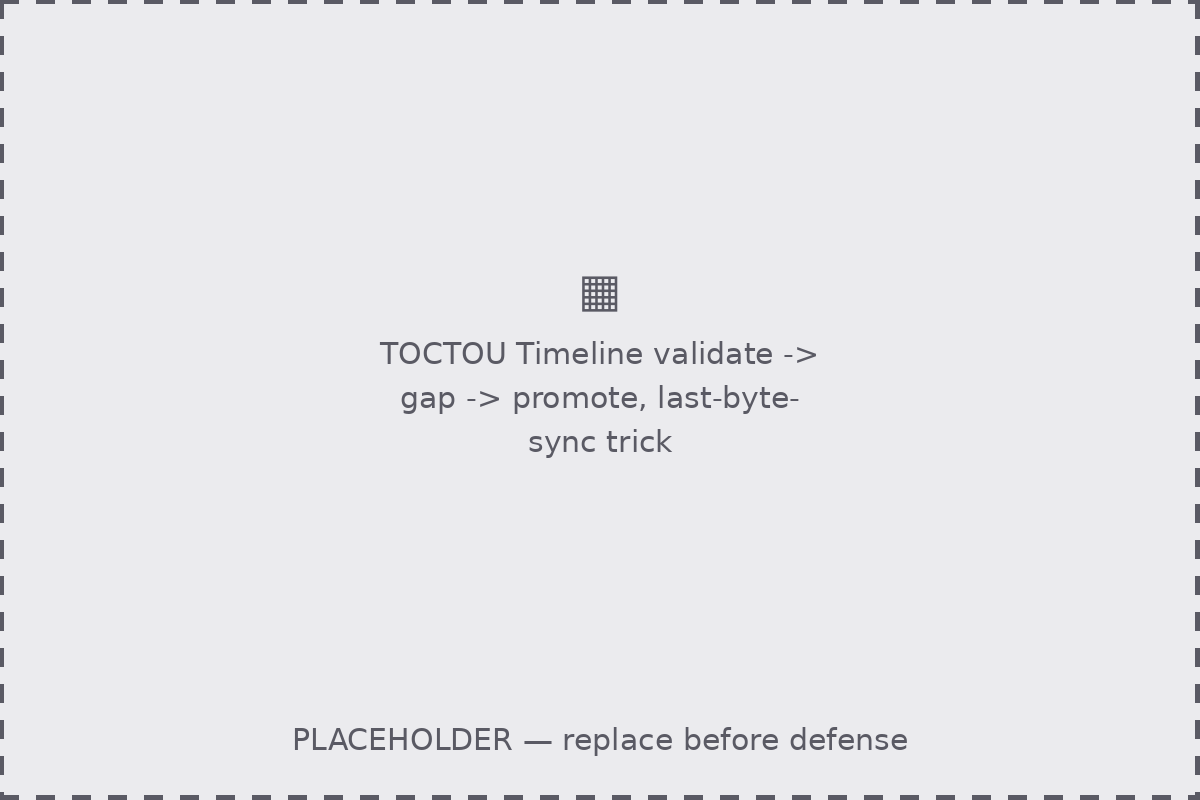
\includegraphics[width=\textwidth]{race-condition-diagram.png}
            \end{column}
        \end{columns}
    \end{frame}

    \begin{frame}{DOM Clobbering}{HTML that overwrites JavaScript}
        \begin{columns}[T]
            \begin{column}{.55\textwidth}
                \begin{itemize}
                    \item Named HTML elements become global JS variables
                    \item \texttt{id="x"} can clobber \texttt{window.x} if \texttt{x} is undefined
                    \item No \texttt{<script>} tag needed --- pure markup
                    \item Sanitizers that allow forms/ids don't stop this
                    \item Trusted script's own config lookup gets redirected
                \end{itemize}
            \end{column}
            \begin{column}{.4\textwidth}
                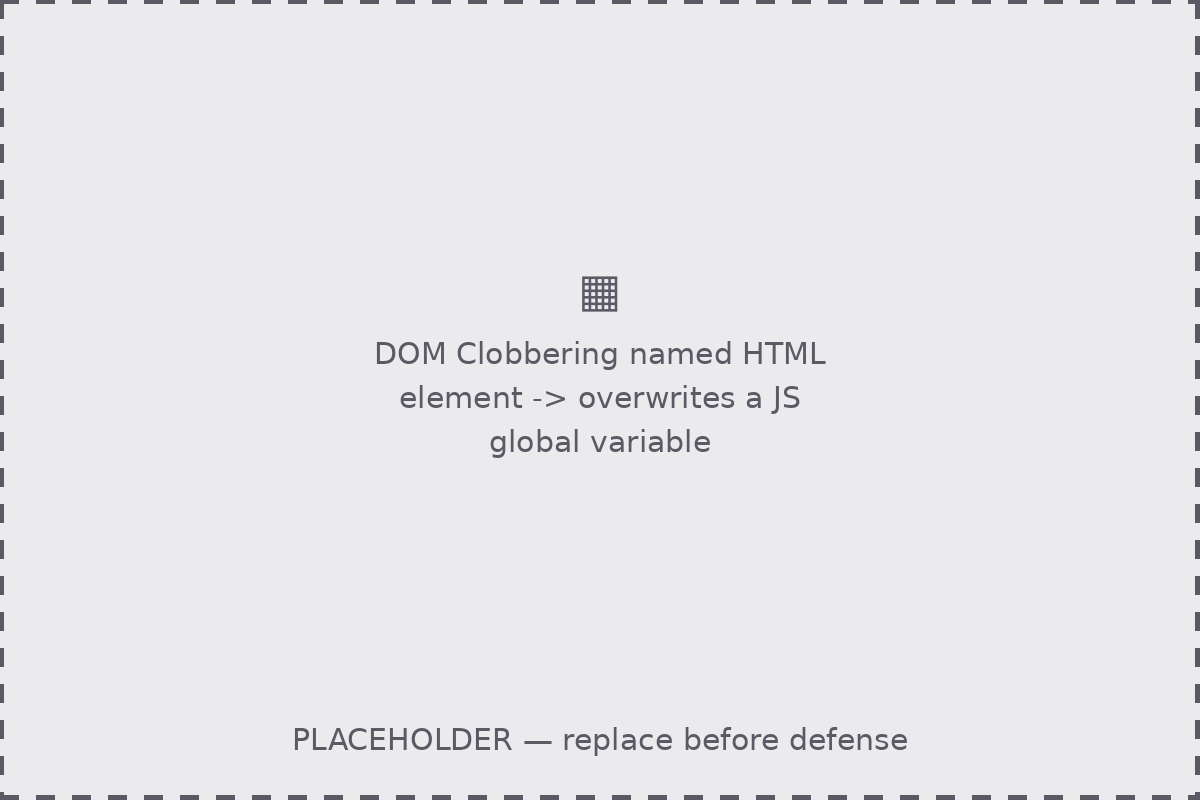
\includegraphics[width=\textwidth]{dom-clobbering-diagram.png}
            \end{column}
        \end{columns}
    \end{frame}

    \begin{frame}{Insecure Deserialization}{When data becomes code}
        \begin{columns}[T]
            \begin{column}{.55\textwidth}
                \begin{itemize}
                    \item Serialize: object $\rightarrow$ bytes. Deserialize: bytes $\rightarrow$ object
                    \item Some formats let bytes pick \emph{which class} to build
                    \item PyYAML's \texttt{yaml.Loader}: builds arbitrary Python objects
                    \item \texttt{!!python/object/apply} tag $\rightarrow$ calls a function directly
                    \item \texttt{yaml.safe\_load}: plain data types only, no tags
                \end{itemize}
            \end{column}
            \begin{column}{.4\textwidth}
                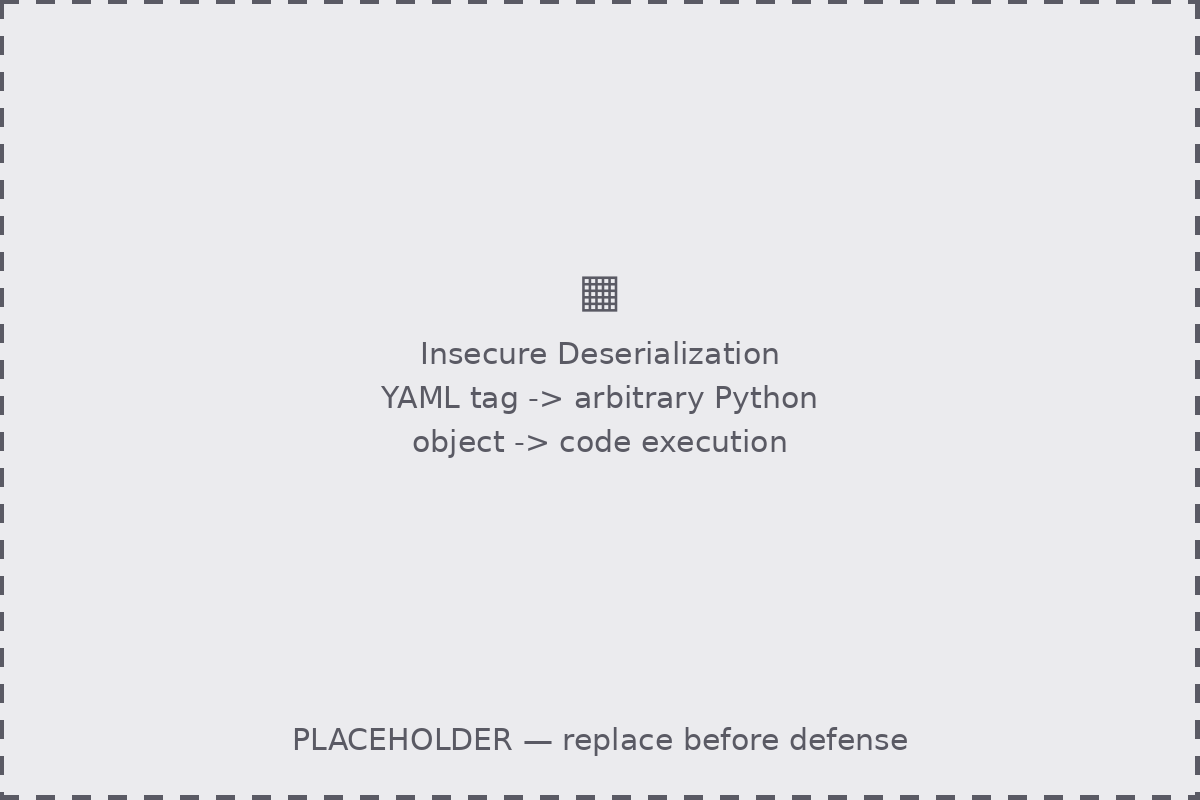
\includegraphics[width=\textwidth]{deserialization-diagram.png}
            \end{column}
        \end{columns}
    \end{frame}

\section{Challenge Architecture}
    \begin{frame}{Two-Tier Deployment}
        \begin{columns}[T]
            \begin{column}{.55\textwidth}
                \begin{itemize}
                    \item Web Pod (Flask) + DB Pod (Postgres)
                    \item \texttt{Kind} cluster, fully portable
                    \item Flag lives only inside Postgres
                \end{itemize}
            \end{column}
            \begin{column}{.4\textwidth}
                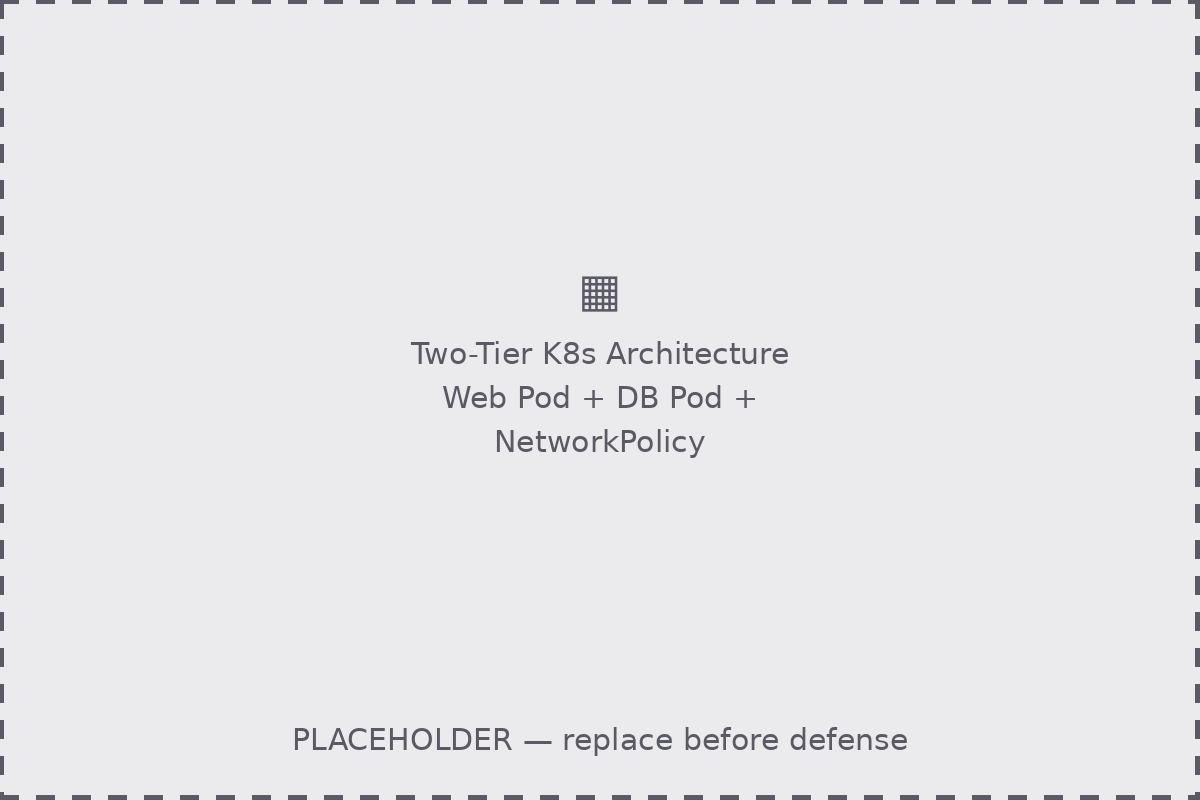
\includegraphics[width=\textwidth]{architecture-diagram.png}
            \end{column}
        \end{columns}
    \end{frame}

    \begin{frame}{Defenses In Place}
        \begin{itemize}
            \item \texttt{readOnlyRootFilesystem: true}
            \item \texttt{NetworkPolicy}: DB ingress from Web Pod only
            \item \texttt{emptyDir}: \texttt{/app/cache}, \texttt{/tmp}
            \item Goal: block the trivial shells and bypasses
        \end{itemize}
    \end{frame}

\section{The Kill Chain}
    \begin{frame}{Overview}
        \begin{center}
            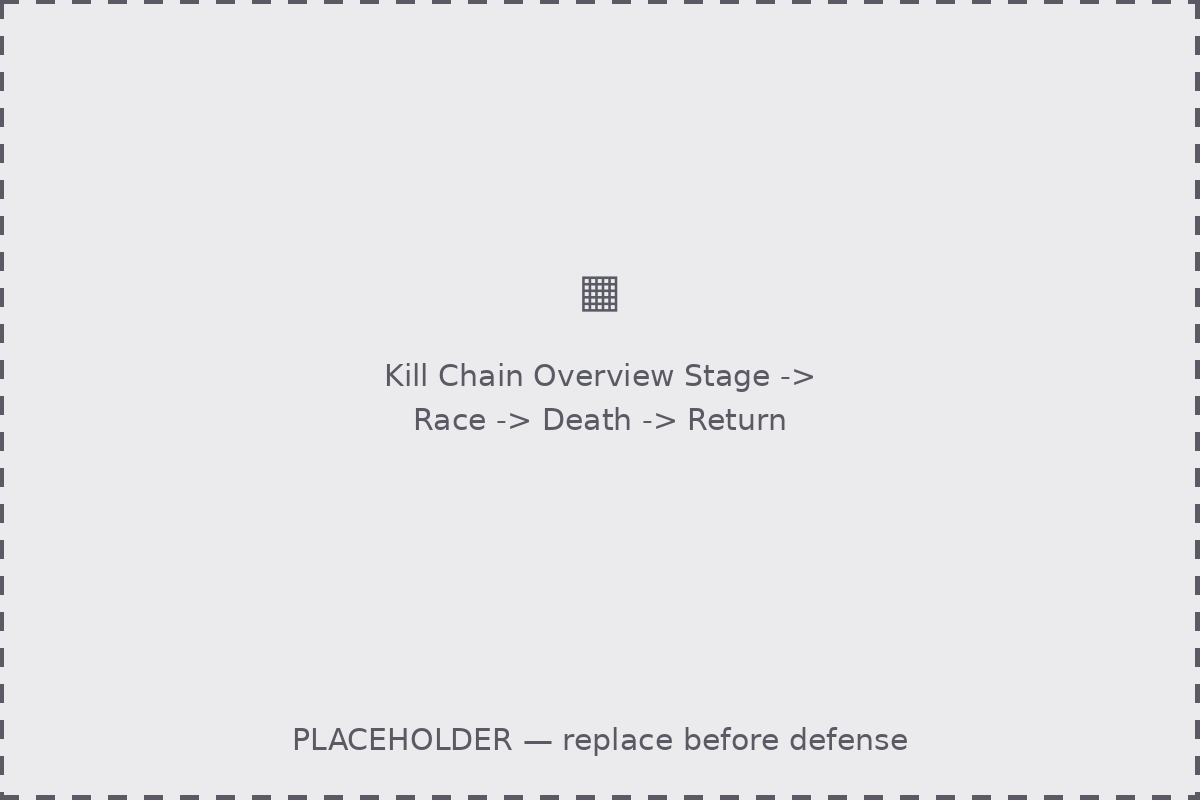
\includegraphics[width=.7\paperwidth]{killchain-diagram.png}
        \end{center}
    \end{frame}

    \begin{frame}{Stage 1 --- Payload Staging}
        \begin{itemize}
            \item Register a standard account
            \item Upload malicious \texttt{profile.yml} as a "backup"
            \item Lands in \texttt{profile.staging.yml} only
        \end{itemize}
    \end{frame}

    \begin{frame}{Stage 2 --- The Race}
        \begin{itemize}
            \item \texttt{/health} validates the staged file (\texttt{safe\_load})
            \item Promotion re-reads the file from disk
            \item Race: swap in the payload after validation, before promotion
        \end{itemize}
    \end{frame}

    \begin{frame}{Stage 3 --- The Death}
        \begin{itemize}
            \item Bio clobbers \texttt{window.STEWARD\_STATUS\_CONFIG}
            \item Support ticket $\rightarrow$ admin bot visits profile
            \item Clobbered fetch hits \texttt{/maintenance/restart}
            \item Pod calls \texttt{os.\_exit(1)}
        \end{itemize}
    \end{frame}

    \begin{frame}{Stage 4 --- The Return}
        \begin{itemize}
            \item Kubernetes restarts the container; \texttt{emptyDir} survives
            \item Boot sequence deserializes \texttt{profile.yml} with \texttt{yaml.Loader}
            \item \texttt{DatabaseExporter} gadget fires
            \item SQL query travels the allowed NetworkPolicy path
            \item Flag POSTed to an external webhook
        \end{itemize}
    \end{frame}

\section{Design Rationale}
    \begin{frame}{Anti-Slop Design}
        \begin{itemize}
            \item Fake metrics / logs / node-status endpoints
            \item Scanners chase SSRF and RCE that isn't there
            \item \texttt{safe\_load} blocks the "obvious" upload
            \item Forces understanding, not guessing
        \end{itemize}
    \end{frame}

    \begin{frame}{Reliability}
        \begin{itemize}
            \item Race outcome is probabilistic, not deterministic
            \item Solve script retries in bursts
            \item Waits for Pod recovery between attempts
            \item Designed to converge eventually, every time
        \end{itemize}
    \end{frame}

\section{Demo}
    \begin{frame}{Live Demo}
        \begin{center}
            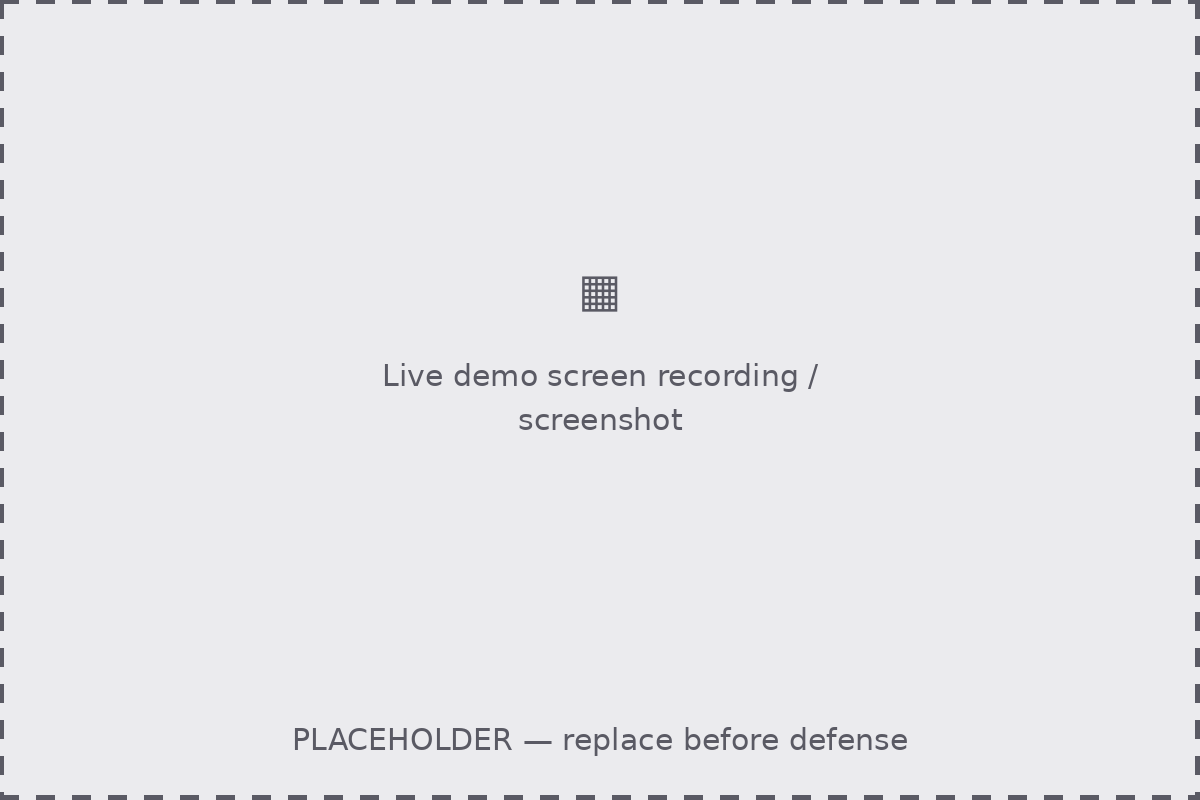
\includegraphics[width=.7\paperwidth]{demo-screenshot.png}
        \end{center}
    \end{frame}

    \begin{frame}
        \insertthankyou
    \end{frame}


\end{document}
